\section{Datenstrukturen und Schnittstellen} 

Abbildung~\ref{Klassendiagramm} bildet die Klassen und Interfaces und alle Daten und Funktionen ab , die zum Durchführen eines Ligrettospiels notwendig sind.

% Bewertungsmassstab:
%  - Sind die Daten vollständig beschrieben, d.h. Anzahl und Wertebereich angegeben (3 Punkte)?
%    - Es sind alle Klassen/Structs anzugeben bis zur den von der Sprache unterstützten Datentypen. 
%      In RPC also int, string etc., in RMI List, Hash, Map etc.


\begin{figure}[H]
	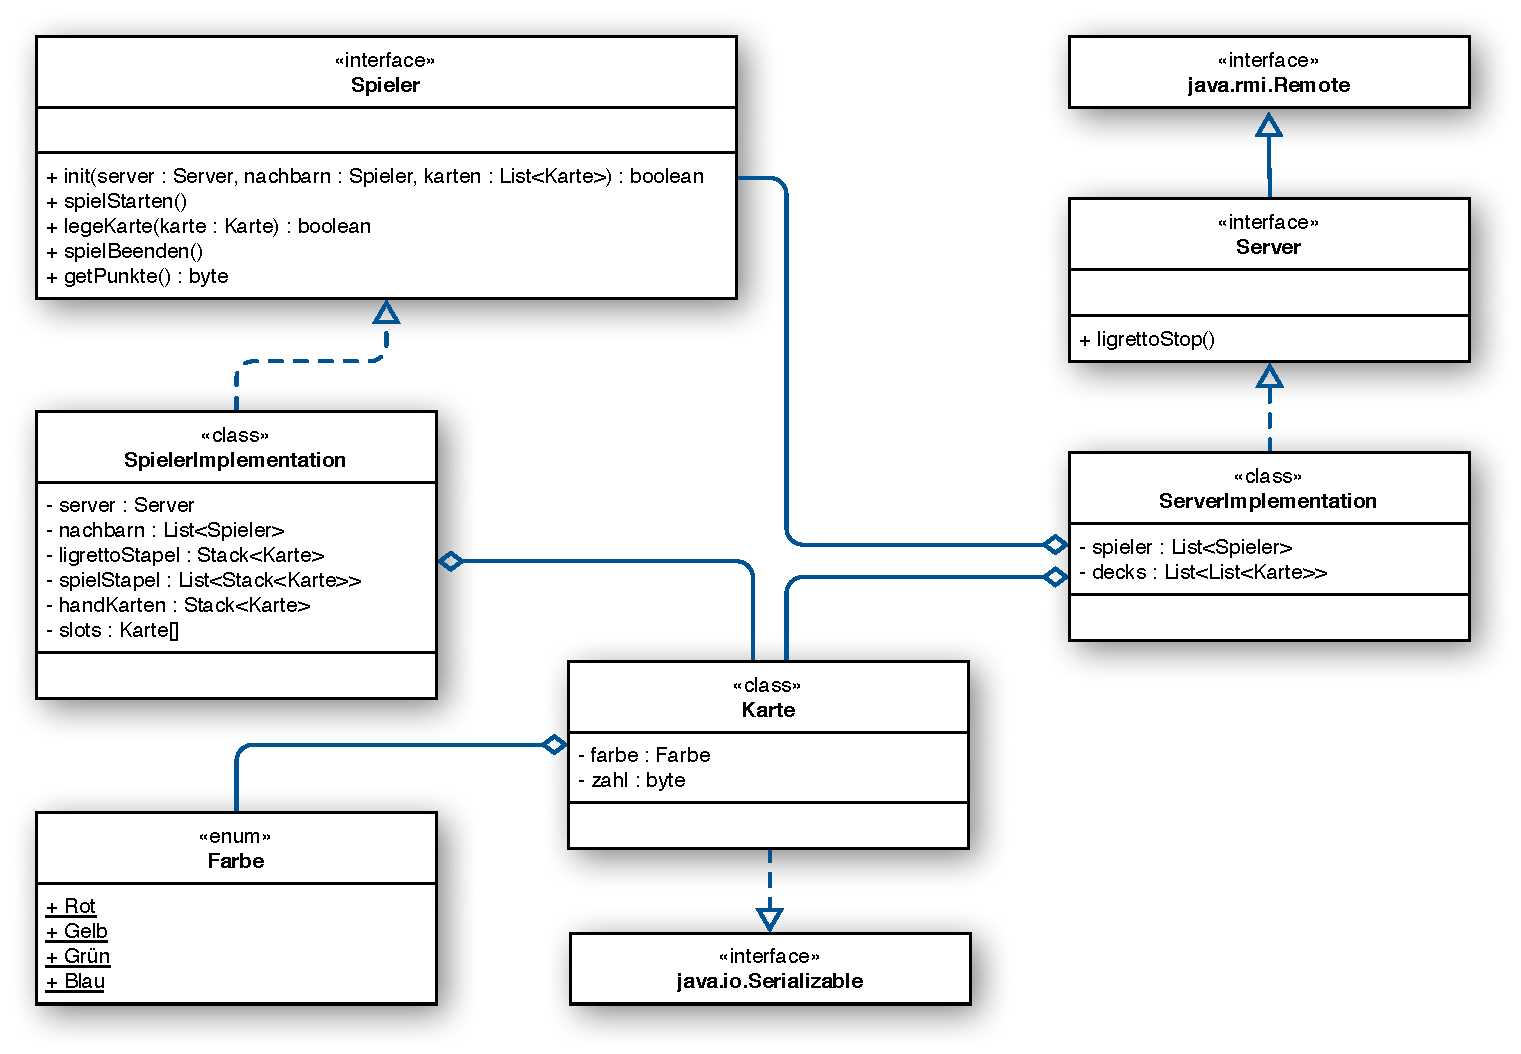
\includegraphics[width=1.0\textwidth,angle=0]{graphics/klassendiagramm.pdf}
	\caption{Klassendiagramm \hfill{} }
	\label{Klassendiagramm}
\end{figure}


\subsection{Karte}

Die Karte hat eine {\bf Farbe} (Rot, Gelb, Grün oder Blau) und eine {\bf Zahl} (zwischen eins und zehn). Sie ist ein serialisierbares Objekt, das zwischen dem Server und verschiedenen Spielern ausgetauscht werden kann.

\lstinputlisting{listings/Karte.java}


\subsection{Server}

Das Serverinterface definiert eine Methode {\bf ligrettoStop()}, welche von dem Spieler, der als erster alle Karten seines Ligrettostapels verspielt hat, aufgerufen wird.

\lstinputlisting{listings/Server.java}

Die Klasse ServerImplementation besitzt zwei Listen; {\bf spieler}, worin alle am Spiel teilnehmenden Spieler enthalten sind und {\bf decks}, welche bereits gemischte Kartenstapel à 40 Karten für die Spieler enthält.

\lstinputlisting{listings/ServerImplementation.java}


\subsection{Spieler}

Ein Spieler kennt vier Methoden. Mit dem Aufruf von {\bf init()} erhält er alle Informationen, die er zum Spiel kennen muss. Wer ist der Server? Wer sind meine Nachbarn? Was sind meine Karten? Dabei werden die 40 Karten gemäss den Spielregeln auf Ligretto-, Spiel- und Handkartenstapel sowie auf die vier Slots aufgeteilt. Das Spiel wird mit {\bf spielStarten()} begonnen. Ab diesem Aufruf spielt der Spieler bis er oder ein Gegner das Spiel beendet. Die Methode {\bf legeKarte()} kann vom Spieler selbst oder von einem seiner Nachbarn aufgerufen werden. Dabei wird eine Karte übergeben und, wenn sie auf einen der Spielstapel passt, niedergelegt. Im Erfolgsfall wird dabei true zurückgegeben, ansonsten false. Ein Aufruf von {\bf spielBeenden()} beendet das Spiel. Zuletzt wird {\bf getPunkte()} vom Server aufgerufen um den Sieger der aktuellen Spielrunde zu ermitteln.

\lstinputlisting{listings/Spieler.java}

SpielerImplementation implementiert das eben beschriebene Spielerinterface. Dabei werden folgende Attribute definiert: {\bf server} - die Serverinstanz, die das Spiel kontrolliert. {\bf nachbarn} - eine Liste aller Nachbarn. {\bf ligrettoStapel} - ein Stapel mit anfänglich zehn Karten, die möglichst rasch verspielt werden müssen. {\bf spielStapel} - Die (maximal vier) Stapel, auf die alle Spieler ihre Karten legen können. {\bf handKarten} - der Stapel mit den Karten, die der Spieler in der Hand hält. {\bf slots} - die vier offen liegenden Karten, die neben dem Ligrettostapel platziert werden.

\lstinputlisting{listings/SpielerImplementation.java}



